\chapter*{Anhang}\label{appendix}
\addcontentsline{toc}{chapter}{Anhang}
\thispagestyle{fancy}
\vspace{1cm}
\begin{figure}[htbp]
    \caption{Statusverlauf visualisiert mit \textit{NagVis}}
    \label{app:nag}\vspace{0.2cm}
    \centering
    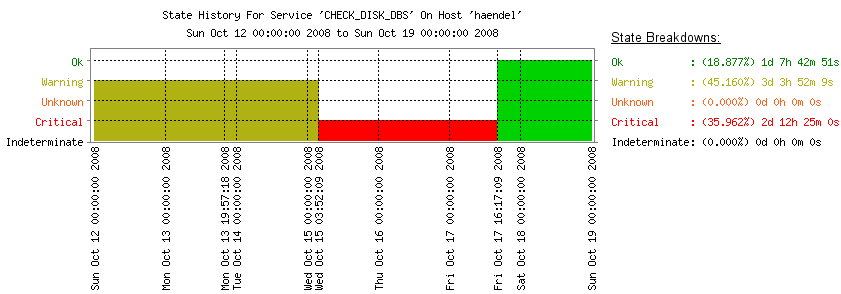
\includegraphics[scale=0.5]{img/nag_trend}  
\end{figure}

\vspace{4cm}
\begin{figure}[h]
    \caption{\textit{liblognorm} - Regel}
    \label{app:liblognorm-rule}\vspace{0.2cm}
    \centering
\begin{minipage}{0.8\textwidth}
\begin{minted}[mathescape,bgcolor=shadecolor]{perl6}
rule=SSHSUCCESS : Accepted password for %user:
word% from %ip:ipv4% port %port : number% %protocol:word%

rule=SSHFAILURE : Failed password for %user:
word% from %ip:ipv4% port %port : number% %protocol:word%

rule=SSHFAILURE : Failed password for invalid user %user:
word% from %ip:ipv4% port %port : number% %protocol:word%

\end{minted}
\end{minipage}
\end{figure}


\begin{figure}[h]
    \caption{\textit{liblognorm} - strukturierte Daten (JSON)}
    \label{app:liblognorm-normalisation}\vspace{0.2cm}
    \centering
    \begin{minipage}{0.8\textwidth}
\begin{minted}[mathescape,bgcolor=shadecolor]{json}
        
{   "data": {
        "protocol":"ssh2",
        "port" : "54548",
        "ip": "10.0.23.4",
        "user": "root"
    },
    "time":"2014-01-29T16:06:00.000",
    "host":"test.example.com",
    "facility":"auth",
    "severity":"info",
    "program" :"sshd",
    "message":" Failed password for root from
                10.0.23.4 port 54548 ssh2",
    "tags" : ["SSHFAILURE"] }
\end{minted}
\end{minipage}
\end{figure}


\begin{figure}[h]
    \caption{\textit{Drools} Brute Force - Regel}
    \label{app:drools-warning}\vspace{0.2cm}
    \centering
    \begin{minipage}{0.8\textwidth}
\begin{minted}[mathescape,bgcolor=shadecolor]{java}
        rule "SSH brute-force attempt"
        no-loop
        when
            Message (   $host:host,
                        $user:data["user"])
            $atts: CopyOnWriteArrayList(size >= 10)
                from collect(
                    Message(    tags contains"SSHFAILURE",
                                host == $host,
                                data["user" ] == $user)
                    over window : time (1m))
        then
            Message last = (Message) $atts.get($atts.size( )-1) ;
        
            for (Object f: $atts) {
                retract ( f ) ;
        }
        
            insert (messageFactory(last)
                . setTime(last.getTime( ))
                . setSeverity(Message.Severity.WARNING)
                . setFacility(Message.Facility.SECURITY)
                . setMessage("SSH brute-force attack" +
                    "for @{data.user} from @{data.ip}")
                . addTag ("BRUTEFORCE")
                . message( )) ;
        end        
        
\end{minted}
\end{minipage}
\end{figure}

\begin{figure}[h]
    \caption{\textit{Drools} - login detection Regel}
    \label{app:drools-emergency}\vspace{0.2cm}
    \centering
    \begin{minipage}{0.8\textwidth}
\begin{minted}[mathescape,bgcolor=shadecolor]{java}
       rule "Successful SSH brute-force attack"
       no-loop
       when
            $ att: Message (    tags contains "SSHFAILURE",
                                tags contains "BRUTEFORCE",
                                $host: host ,
                                $user: data ["user"])
            $ suc: Message (    host == $host,
                                data ["user" ] == $user,
                                tags contains "SSHSUCCESS",
                                this finishes[10 s] $att)
       then
            $att.addTag("INCIDENT");
            $att.setSeverity(Severity.EMERGENCY);
            $att.setMessage($att.getMessage( ) + "[bruteforce]");
       update ($att);
       end
        
\end{minted}
\end{minipage}
\end{figure}

\begin{figure}[htbp]
    \caption{Aufbau des verwendeten ELK-Stacks}
    \label{app:demo-elk}\vspace{0.2cm}
    \centering
    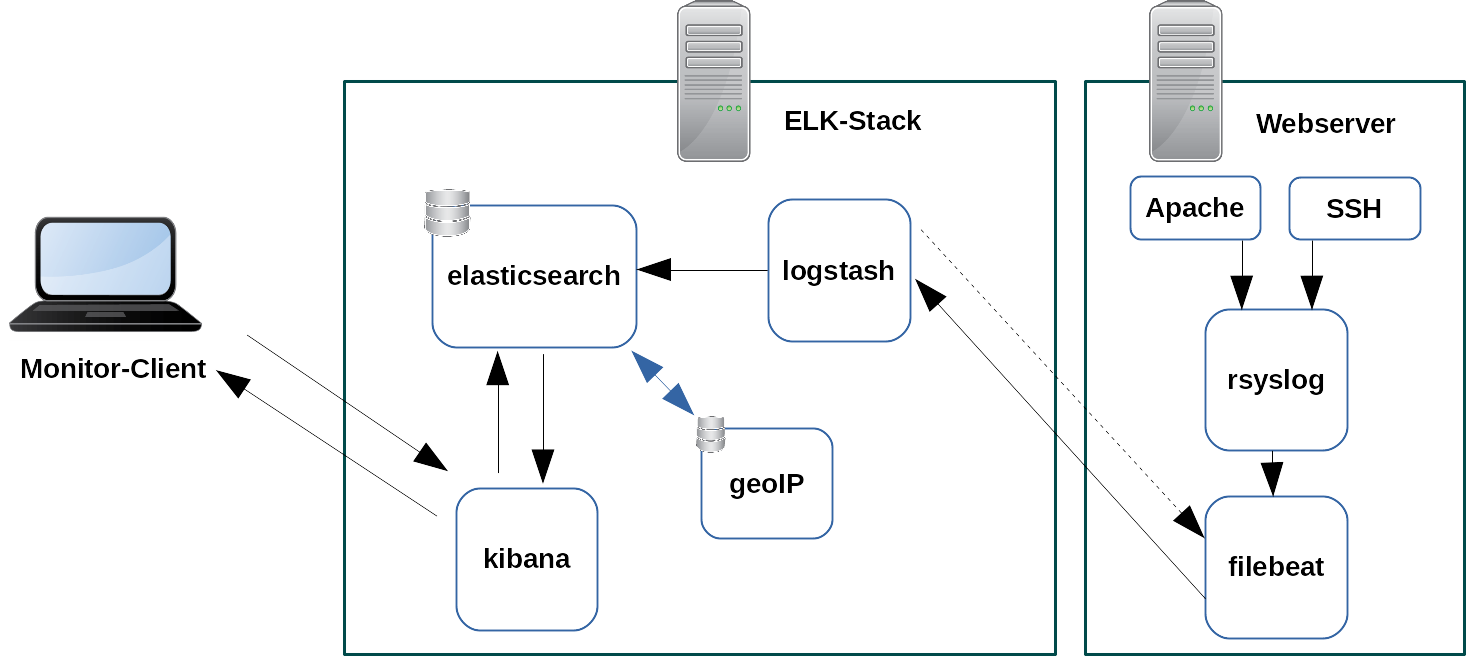
\includegraphics[scale=0.33]{img/demo-elk}  
\end{figure}